% This work is licensed under the Creative Commons Attribution-NonCommercial 4.0 International License.
% To view a copy of this license, visit http://creativecommons.org/licenses/by-nc/4.0/
% or send a letter to Creative Commons, PO Box 1866, Mountain View, CA 94042, USA.

% !TEX TS-program = xelatex

\documentclass[../Main/chem331-notes.tex]{subfiles}
\begin{document}

\setcounter{section}{1}
\section{The Bohr model of the hydrogen atom}

\subsection{The classical model of the hydrogen atom}
The hydrogen atom ($^1$H) is composed of two particles, an electron (with mass $m_e$) and a proton (with mass $M_p$).
The ratio of the two masses is $M_p/m_e \approx 1836$, that is, the electron is significantly lighter than the proton.
So we will ignore the motion of the proton and assume that it has a fixed position in space, which for convenience we assume to be the origin of a 3D Cartesian coordinate system.\mnote{This approximation is not necessary, as we will see later, we can work in a set of reduced coordinates and treat both the motion of the proton and the electron.}
In this case the classical energy expression for the electron orbiting around the proton is given by the sum of the kinetic and potential energy of the electron
\begin{equation}
E = \underbrace{\frac{1}{2} m_e v^2}_{\text{Kinetic energy}}
+ \underbrace{\frac{1}{4 \pi \epsilon_0} \frac{q_e q_p}{r}}_{\text{Potential energy}},
\end{equation}
where $q_e$ and $q_p$ are the charge of the electron and proton, respectively, and $\epsilon_0$ is the vacuum permittivity.\mnote{$\epsilon_0 = 8.854187817 \times 10^{-12} \, \si{\farad} \cdot \si{\meter}^{-1}$.}
If we write the charge of the electron\mnote{Be careful to avoid confusing this with Euler's number $e = 2.718281\ldots$.} as $q_e = -e$ then the charge of the proton is $q_p = e$ and the energy may be written as
\begin{equation}
E = \frac{1}{2} m_e v^2 - \frac{1}{4 \pi \epsilon_0} \frac{e^2}{r},
\end{equation}

Assuming that the electron is in a stationary circular orbit, the force accelerating it towards the nucleus has magnitude
\begin{equation}
f_a = \frac{m_e v^2}{r}.
\end{equation}
This force must be equal to the Coulomb force attracting the electron to the proton
\begin{equation}
f_c =  \frac{1}{4 \pi \epsilon_0} \frac{e^2}{r^2}.
\end{equation}
For a stationary orbit the force due to acceleration and the Coulomb force must match, so after equating the two expressions we get
\begin{equation}
\label{eq:stationary_condition}
m_e v^2 = \frac{1}{4 \pi \epsilon_0} \frac{e^2}{r}.
\end{equation}
Plugging this equation in the energy expression we get
\begin{equation}
E = \frac{1}{2} \frac{1}{4 \pi \epsilon_0} \frac{e^2}{r} - \frac{1}{4 \pi \epsilon_0} \frac{e^2}{r}= - \frac{1}{2} \frac{1}{4 \pi \epsilon_0} \frac{e^2}{r}.
\end{equation}
This equation relates the energy of an orbit ($E$) to the distance of the electron from the proton ($r$).

\begin{exercise}
What does the spectrum for the classical hydrogen atom look like?
\end{exercise}

\marginpar{
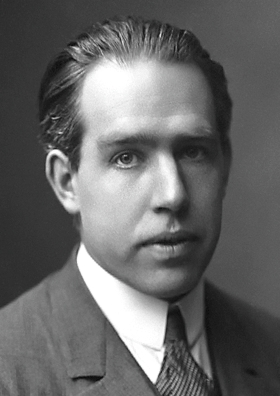
\includegraphics[width=1.5in]{../Figures/Niels_Bohr.jpg}
\captionof{figure}{Niels Bohr.}
}

\subsection{Bohr's model}
The classical model of the hydrogen atom fails at describing the discrete nature of the spectrum observed in experiments.
Bohr's solution to this problem involved postulating that certain physical quantities can only take certain values.\mnote{Physicist Niels Bohr (Denmark, 1885--1962).}
Recall that the angular momentum of particle is defined as $\mathbf{L} = \mathbf{r} \times \mathbf{p} = m \mathbf{r} \times \mathbf{v}$, where $\mathbf{r}$ is the vector position of a particle, $m$ is its mass, $\mathbf{p}$ its momentum vector, and $\mathbf{v}$ is its velocity.
For an electron orbiting around the proton the magnitude of angular momentum is
\begin{equation}
L = r m_e v.
\end{equation}
Bohr assumed that this quantity is allowed to take only the following values
\begin{iequation}
L = n \frac{h}{2\pi} = n\hbar \quad n = 1, 2, 3, \ldots.
\end{iequation}
Note that the quantity $\frac{h}{2\pi}$ appears so often in quantum mechanics that it is convenient to introduce a symbol for it, $\hbar = \frac{h}{2\pi}$, which we refer to as ``h-bar.''
Combining the two expressions for the angular momentum we obtain
\begin{equation}
r m_e v = n\hbar \Rightarrow v = \frac{n\hbar}{r m_e}
\end{equation}
Combining this condition with the stationary condition for the hydrogen atom [Eq.~\eqref{eq:stationary_condition}] we get
\begin{equation}
m_e \left(\frac{n\hbar}{r m_e}\right)^2 = \frac{1}{4 \pi \epsilon_0} \frac{e^2}{r},
\end{equation}
which we can write as
\begin{equation}
\label{eq:bohr:radius}
r = \frac{4 \pi \epsilon_0 n^2\hbar^2}{e^2 m_e}, \quad n = 1, 2, 3, \ldots .
\end{equation}
These are the allowed values of the orbit radii for the electron in the Bohr model.

We can now use this expression to determine the allowed energy levels.
Taking the equation for $r$ [Eq.~\eqref{eq:bohr:radius}] and plugging it in the energy expression we get
\begin{iequation}
E_n = - \frac{m_e e^4}{32 n^2\hbar^2 \pi^2 \epsilon_0^2 }, \quad n = 1, 2, 3, \ldots .
\end{iequation}
This equation predicts discrete energy levels, and these turn out to be remarkably accurate.

\marginpar{
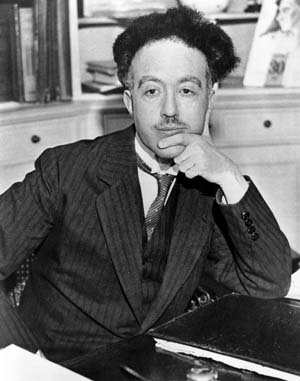
\includegraphics[width=1.5in]{../Figures/Louis_de_Broglie.jpg}
\captionof{figure}{Louis de Broglie.}
}

\subsection{Rydberg's formula}
Next we will derive an expression (Rydberg's formula) that tells us what is the energy difference between energy levels of the hydrogen atom.
Consider a transition from level $n_1$ to $n_2$.
The energy difference $E_{n_2} - E_{n_1}$ is then given by
\begin{equation}
\Delta E = E_{n_2} - E_{n_1} = - \frac{m_e e^4}{32\hbar^2 \pi^2 \epsilon_0^2 } \left(\frac{1}{n_1^2} - \frac{1}{n_2^2} \right).
\end{equation}
Another common way to report this equation is to convert it to wavenumbers\mnote{When converting from $\si{\meter}$ to $\si{\per\centi\meter}$ remember that $\SI{1}{\meter} = \SI{100}{\centi\meter}$, hence, $\SI{1}{\per\meter} = \SI{0.01}{\per\centi\meter}$.}
\begin{iequation}
\bar{\nu} = \frac{\Delta E}{hc} = R_\infty \left(\frac{1}{n_2^2} - \frac{1}{n_1^2} \right),
\end{iequation}
where $R_\infty$ is Rydberg's constant ($R_\infty \approx \SI{109737.31568508}{\per\centi\meter}$).

\subsection{de Broglie's hypothesis}
Louis de Broglie's\mnote{Physicist Louis de Broglie (France, 1892--1987).}

 contribution to the understanding of the spectrum of the hydrogen atom is the hypothesis that in the same way we assign a wavelength to photons (light), we can also assign a wavelength to particles (matter).
Starting with Einsteins's result
\begin{equation}
E^2 = (cp)^2 + (m_0 c^2)^2,
\end{equation}
where $p$ is the momentum of a particle and $m_0$ is its rest mass, we can derive for photons ($m = 0$) that
\begin{equation}
E = pc.
\end{equation}
However, from Einstein we also know that photons carry an amount of energy equal to $E = h \nu$, so that equating these two expressions for the energy we derive
\begin{equation}
pc = h \nu \Rightarrow pc = \frac{hc}{\lambda}  \Rightarrow p = \frac{h}{\lambda}.
\end{equation}
de Broglie's point is that this result should be extended also to particles, so that for a particle we can write
\begin{iequation}
\lambda = \frac{h}{p}.
\end{iequation}

We can now apply de Broglie's hypothesis to understand the quantization of angular momentum in the hydrogen atom.
As shown in the figure below we require that as the electron orbits the de Broglie wave associated with it must go through an integer number of cycles every time it orbits around the proton. 
\begin{figure}[htbp]
   \centering
   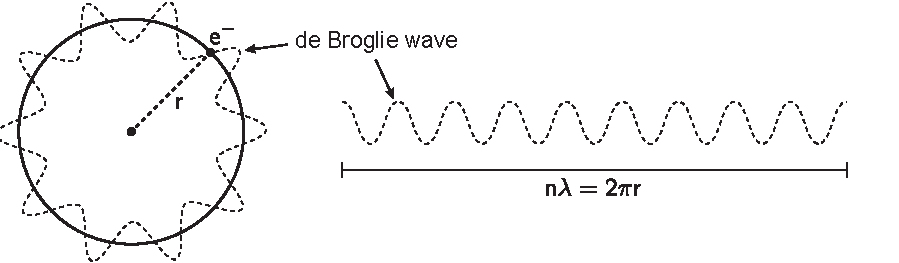
\includegraphics[width=4in]{../Figures/deBroglieWave.pdf} % requires the graphicx package
%   \caption{example caption}
%   \label{fig:example}
\end{figure}

This condition is equivalent to equating the circumference of the orbit ($ 2 \pi r$) with a integer multiple of the wavelength
\begin{equation}
n \lambda = 2 \pi r.
\end{equation}
From this result and de Broglie's formula we derive,
\begin{equation}
n \frac{h}{p} = 2 \pi r
\end{equation}
which may be used to find the magnitude of angular momentum for the electron
\begin{equation}
\label{eq:bohr:angular_momentum}
L = r p = \frac{n h}{2 \pi}.
\end{equation}
 This shows that the de Broglie's formula can be used to rationalize Bohr's hypothesis.
 
 \marginpar{
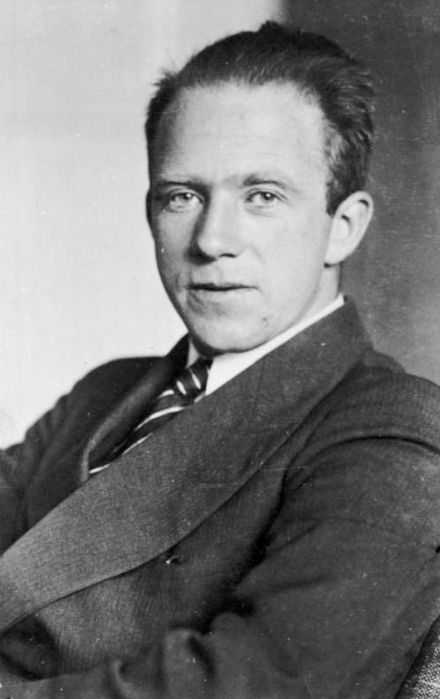
\includegraphics[width=1.5in]{../Figures/Werner_Heisenberg.jpg}
\captionof{figure}{Werner Heisenberg.}
}

\begin{exercise}
What are the allowed values of $n$ in Eq.~\eqref{eq:bohr:angular_momentum}? Why?
\end{exercise}

\subsection{Heisenberg's uncertainty principle}
How can better understand the dual nature (particle/wave) of matter particles like electrons?
Heisenberg proposed that there is an intrinsic limit to the precision with which we can measure certain physical quantities (uncertainty principle).
\mnote{After physicist Werner Heisenberg (Germany, 1901--1976).}

For a particle moving in one dimension, the uncertainty principle states that the uncertainty in the position ($\Delta x$) times the uncertainty in the momentum ($\Delta p$) must be greater than or equal to a constant
\begin{iequation}
\Delta x \Delta p \geq \frac{\hbar}{2}.
\end{iequation}
So, if position is measured with high accuracy, then the uncertainty on the momentum of the particle will become very large.
Similarly, if we know the momentum of an object with high accuracy, the uncertainty on the position will be come large.
Note that since momentum is $p = mv$, we can then write the uncertainty in the position as
\begin{equation}
\Delta x \geq \frac{\hbar}{2 m \Delta v}.
\end{equation}
So the uncertainty principle implies that for equal  uncertainty in the velocity $\Delta v$, lighter object have greater uncertainty in the position.
In our common experience we deal with macroscopic objects whose weight is order of magnitudes larger than that of electrons and protons.
In our common experience we deal with macroscopic objects whose weight is order of magnitudes larger than that of electrons and protons and we do not experience the wave-like nature of matter.
For example, the uncertainty on the position of a laptop ($m \approx \SI{1}{\kilo\gram}$) falling at a speed of \SI{1}{\meter\per\second} with an uncertainty in the velocity of  \SI{0.01}{\meter\per\second} is
\begin{equation}
\Delta x \geq \frac{\hbar}{2 \cdot 1 \cdot 0.01} \approx 10^{-32} \si{\meter},
\end{equation}
which is a minuscule number. In the case of an electron ($m_e = $) we instead find that the uncertainty is much larger, of the order of a centimeter
\begin{equation}
\Delta x \geq \frac{\hbar}{2 \cdot 9.1 \cdot 10^{-31} \cdot 0.01} \approx 0.01 \si{\meter}.
\end{equation}
The uncertainty principle then explains why we do not experience the wave-like nature of macroscopic objects.

\end{document}